\documentclass[ignorenonframetext, professionalfonts, hyperref={pdftex, unicode}]{beamer}

\usetheme{Copenhagen}
\usecolortheme{wolverine}

%Packages to be included
%\usepackage{graphicx}

\usepackage[russian]{babel}
\usepackage[utf8]{inputenc}
\usepackage[T1]{fontenc}

%%\usepackage[orientation=landscape, size=custom, width=16, height=9.75, scale=0.5]{beamerposter}

\usepackage{textcomp}

\usepackage{beamerthemesplit}

\usepackage{ulem}

\usepackage{verbatim}

\usepackage{ucs}


\usepackage{listings}
\lstloadlanguages{bash}

\lstset{escapechar=`,
	extendedchars=false,
	language=sh,
	frame=single,
	tabsize=2, 
	columns=fullflexible, 
%	basicstyle=\scriptsize,
	keywordstyle=\color{blue}, 
	commentstyle=\itshape\color{brown},
%	identifierstyle=\ttfamily, 
	stringstyle=\mdseries\color{green}, 
	showstringspaces=false, 
	numbers=left, 
	numberstyle=\tiny, 
	breaklines=true, 
	inputencoding=utf8,
	keepspaces=true,
	morekeywords={u\_short, u\_char, u\_long, in\_addr}
	}

\definecolor{darkgreen}{cmyk}{0.7, 0, 1, 0.5}

\lstdefinelanguage{diff}
{
    morekeywords={+, -},
    sensitive=false,
    morecomment=[l]{//},
    morecomment=[s]{/*}{*/},
    morecomment=[l][\color{darkgreen}]{+},
    morecomment=[l][\color{red}]{-},
    morestring=[b]",
}

\author[Epam]{{\bf Epam}\\Low Level Programming Department}

%\institution[EPAM]{EPAM}
%\logo{\includegraphics[width=1cm]{logo.png}}


\title{Введение в GNU/Linux}


%%%%%%%%%%%%%%%%%%%%%%%%%%%%%%%%%%%%%%%%%%%%%%%%%
%%%%%%%%%% Begin Document  %%%%%%%%%%%%%%%%%%%%%%
%%%%%%%%%%%%%%%%%%%%%%%%%%%%%%%%%%%%%%%%%%%%%%%%%




\begin{document}

\begin{frame}
	\frametitle{}
	\titlepage
	\vspace{-0.5cm}
	\begin{center}
	%\frontpagelogo
	\end{center}
\end{frame}


%%%%%%%%%%%%%%%%%%%%%%%%%%%%%%%%%%%%%%%%%   
%%%%%%%%%% Content starts here %%%%%%%%%%
%%%%%%%%%%%%%%%%%%%%%%%%%%%%%%%%%%%%%%%%%

\section{Основы работы с сетевой подсистемой}

\mode<all>{\begin{frame}{Сетевая подсистема Linux}

	\begin{block}{Cетевой интерфейс}

		Сетевой интерфейс в Linux -– это абстрактный именованный объект,  используемый для передачи 
		данных через некоторую линию связи без привязки к ее (линии связи) реализации.
	\end{block}
\end{frame}

\begin{frame}{Сетевая подсистема Linux}

	\center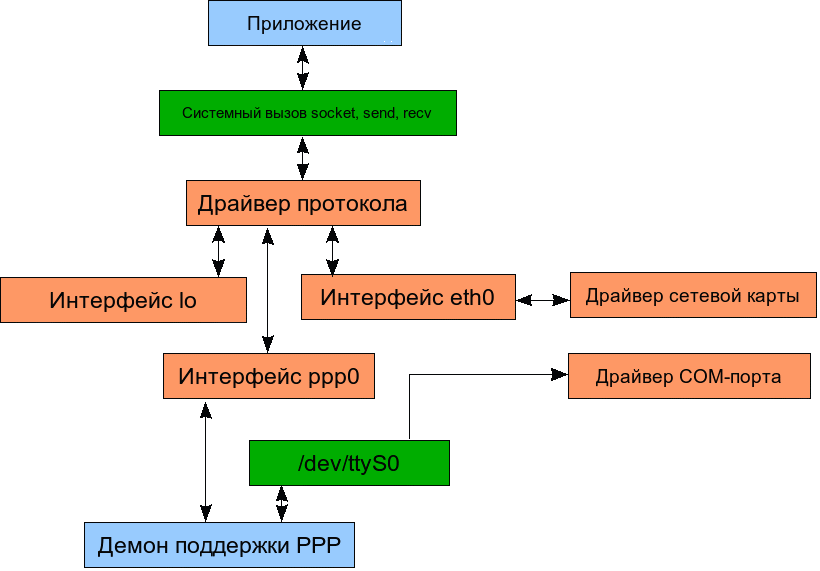
\includegraphics[height=0.8\textheight]{../../slides/networking/06-netstack.png}

\end{frame}


}

\subsection{Управление интерфейсами}
\mode<all>{\begin{frame}{Команды управления настройками сети}
	\begin{itemize}
	  \item ifconfig/route
	  \item iproute2
	\end{itemize}

	\begin{itemize}
		\item Список интерфейсов
			\begin{itemize}
				\item {\tt ifconfig -a}
				\item {\tt ip link show}
			\end{itemize}
		\item Включение интерфейса 
			\begin{itemize}
				\item {\tt ifconfig <iface> up}
				\item {\tt ip link set <iface> up}
			\end{itemize}
	  \item Выключение интерфейса
			\begin{itemize}
				\item {\tt ifconfig <iface> down}
				\item {\tt ip link set <iface> down}
			\end{itemize}
	  \item Назначение адреса
			\begin{itemize}
				\item {\tt ifconfig eth0 192.168.1.17 netmask 255.255.254.0 up}
				\item {\tt ip addr add 192.168.1.17/23 dev eth0}
			\end{itemize}
	\end{itemize}
\end{frame}

\begin{frame}{Конфигурационные файлы}
  \begin{itemize}
    \item {\tt /etc/resolv.conf}
    \item {\tt /etc/hosts}
	\item {\tt /etc/sysconfig/network}
    \item Расположение зависит от дистрибутива:
		\begin{itemize}
			\item RH-like: {\tt /etc/sysconfig/network-scripts}\\
				{\tt /etc/sysconfig/network-scripts/ifcfg-eth0}
			\item ALTLinux: {\tt /etc/net/ifaces}
			\item Debian: {\tt /etc/network/interfaces}
			\item Gentoo: {\tt /etc/conf.d/net}
		\end{itemize}
  \end{itemize}
\end{frame}

\begin{frame}{Дополнительные интерфейсы}
	\begin{block}{Алиасы}
		\begin{itemize}
			\item ifconfig <iface>:<alias> <ip> up
			\item ifconfig <iface> add <ip> up
			\item ip addr add <ip> {\bf label} <iface>:<alias> dev <iface>
		\end{itemize}
	\end{block}
	\pause
	\begin{block}{VLAN}
		\begin{itemize}
			\item vconfig add <iface> <id>
			\item vconfig rem <iface>{\bf.}<id>
			\item ip link add {\bf link} <iface> name <vlan\_name> {\bf type vlan id <id>}
			\item ip link delete <vlan\_name>
		\end{itemize}
	\end{block}

\end{frame}


}

\subsection{Полезные программы}
\mode<all>{\begin{frame}{Полезные утилиты}
	\begin{center}
		\begin{itemize}
			\item netstat / ss
			\item nslookup / dig
			\item ping
			\item traceroute
			\item tcpdump
			\item telnet
			\item netcat
			\item nmap
		\end{itemize}
	\end{center}

\end{frame}


\begin{frame}[allowframebreaks]{Полезные утилиты: практика}

		\begin{block}{netstat}

			Узнать:
			\begin{itemize}
				\item список используемых сокетов
				\item серверных сокетов
				\item имена/pid серверов
				\item узнать номера портов
			\end{itemize}
		\end{block}
	
		\framebreak
		\begin{block}{telnet/netcat}

			\begin{itemize}
				\item Чат по протоколу TCP с соседом
				\item Чат по протоколу UDP с соседом
				\item Передать текстовый и бинарный файлы
			\end{itemize}
	
			При создании чата использовать {\tt netstat} и {\tt tcpdump}
			для получения информации о соединении.
		\end{block}

		\framebreak
		\begin{block}{nmap}
			\begin{itemize}
				\item сканирование соседа
				\item сканирование выделенных портов у соседа (поиск сервера чата) 
				\item узнать список открытых портов на всех машинах в аудитории
				\item узнать список работающих машин
			\end{itemize}
		\end{block}
	
\end{frame}

tcpdump
0. pcap файлы/libpcap
1. запуск монитора
2. запуск чата
3. монитор-фильтр-анализ

}

\section{ssh}
\mode<all>{\begin{frame}{ssh}

	\begin{block}{ssh -- терминал}
		{\tt ssh [user@]host[:port]}\\
		{\tt ssh host [-l user] [-p port]}
		\begin{itemize}
			\item -v -- "разговорчивый" режим 
			\item -t -- насильное назначение псевдотерминала (для автоматизации)
		\end{itemize}
		Вся конфигурация пользователя: {\tt \$HOME/.ssh}
	\end{block}

	\pause

	\begin{block}{... и не только}
		\begin{itemize}
			\item -X -- "проброс" графики 
			\item -L [bindip:]port:rhost:rport -- "пробрасывание" порта с удаленной машины на локальную
			\item -R [bindip:]port:lhost:lport -- "пробрасывание" порта с локальной машины на удаленную
			\item -W host:port -- stdin/stdout с указанным хостом
			\item -D port -- динамический прокси
		\end{itemize}
	\end{block}
\end{frame}


}


\section{Дополнительные типы интерфейсов}

\subsection{alias, vlan}
\mode<all>{
\begin{frame}{Дополнительные интерфейсы}
	\begin{block}{Алиасы}
		\begin{itemize}
			\item ifconfig <iface>:<alias> <ip> up
			\item ifconfig <iface> add <ip> up
			\item ip addr add <ip> {\bf label} <iface>:<alias> dev <iface>
		\end{itemize}
	\end{block}
	\pause
	\begin{block}{VLAN}
		\begin{itemize}
			\item vconfig add <iface> <id>
			\item vconfig rem <iface>{\bf.}<id>
			\item ip link add {\bf link} <iface> name <vlan\_name> {\bf type vlan id <id>}
			\item ip link delete <vlan\_name>
		\end{itemize}
	\end{block}

\end{frame}


}
\subsection{Мосты}
\mode<all>{\begin{frame}{Мосты}
	\begin{itemize}
		\item Создать -- {\tt brctl addbr <bridge>}
		\item Удалить -- {\tt brctl delbr <bridge>}
		\item Добавить интерфейс -- {\tt brctl addif <bridge> <device>}
		\item Удалить интерфейс-- {\tt brctl addif <bridge> <device>}
	\end{itemize}
\end{frame}


}
\subsection{Тоннели}
\mode<all>{
\begin{frame}{''Виртуальные'' интерфейсы}
	\begin{block}{TUN/TAP}

		{\tt modprobe tun}

		\begin{itemize}
			\item Добавить интерфейс TUN -- {\tt tunctl -n -t <ifacename>}
			\item Добавить интерфейс TAP -- {\tt tunctl -p -t <ifacename>}
			\item Удалить интерфейс -- {\tt tunctl -d <ifacename>}
		\end{itemize}
	\end{block}

	\pause

	\begin{block}{Практика}
		\begin{itemize}
			\item Создать интерфейс TAP с именем {\tt mytap}
			\item Создать мост с именем {\tt mybr}
			\item Назначить интерфейсу {\tt mytap} адрес {\tt 192.168.0.<n>/24}
			\item Добавить интерфейсы {\tt mytap} и {\tt eth0} к мосту {\tt mybr}
			\item Запустить {\tt tcpdump} на интерфейсах {\tt mybr} и {\tt mytap}
			\item Запустить {\tt ping} соседа
		\end{itemize}
	\end{block}

\end{frame}


}

\section{Маршрутизация}
\mode<all>{\begin{frame}{Маршрутизация}
	\begin{itemize}
		\item netstat -r
		\item route
		\item ip route show
	\end{itemize}

	\begin{block}{Разрешить маршрутизацию на хосте}
		{\tt echo 1 > /proc/sys/net/ipv4/ip\_forward}
	\end{block}
\end{frame}


}

\section{iptables}
\mode<all>{\begin{frame}{Iptables}

	\center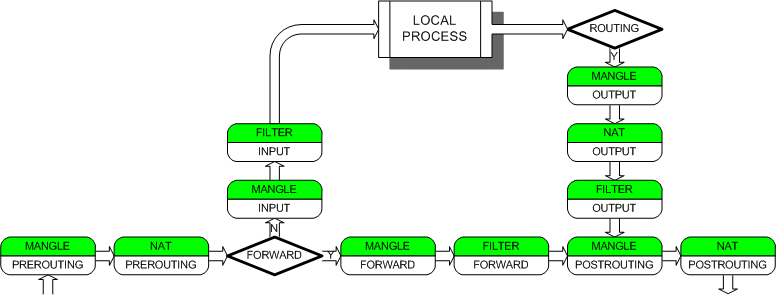
\includegraphics[height=0.4\textheight]{../../slides/networking/06-iptables.png}

	\begin{itemize}
	\begin{columns}
		\column{0.3\textwidth}
			\item[ ] {\bf iptables -L -t <table>}
				\bigskip

			\item filter -- файерволл
				\begin{itemize}
					\item INPUT
					\item FORWARD
					\item OUTPUT
				\end{itemize}
		\column{0.3\textwidth}
			\item nat -- преобразования адресов
				\begin{itemize}
					\item PREROUTING
					\item INPUT
					\item OUTPUT
					\item POSTROUTING
				\end{itemize}
		\column{0.3\textwidth}
			\item mangle -- специальные  изменения  пакетов (TOS, TTL, MARK)
				\begin{itemize}
					\item PREROUTING
					\item INPUT
					\item FORWARD
					\item OUTPUT
					\item POSTROUTING
				\end{itemize}
		\end{columns}
	\end{itemize}

\end{frame}


}

%\mode<all>{\begin{frame}{Практика: создание тестовой среды}

	\center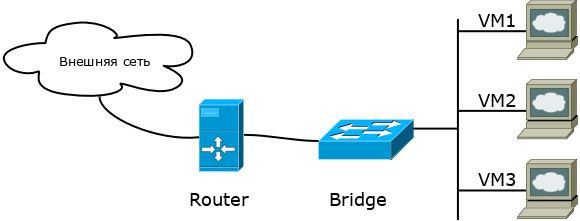
\includegraphics[height=0.4\textheight]{../../slides/networking/net-practice.png}


	\begin{block}{Задача}
		Запустить 3 идентичные виртуальные машины.\\
		Каждой машине назначить адрес из отдельного IP диапазона.\\
		Организовать сетевую ''видимость'' между виртуальными машинами, а также хостом.		
	\end{block}

\end{frame}



\begin{frame}
	\frametitle{Подготовка дисковой подсистемы}
			\begin{itemize}
				\item Создать пустой файл размером в 1.5 GB и отобразить на устройство
					/dev/loop ({\tt dd, losetup})
				\item Создать группу томов на базе этого устройства ({\tt pvcreate, vgcreate})
				\item Выделить 1 GB под логический диск ({\tt lvcreate})
				%\item Скопировать образ виртуального диска в полученный логический том ({\tt dd})
				%\item Создать снимок логического тома на 100MB ({\tt lvcreate}) для каждой виртуальной машины.
			\end{itemize}
\end{frame}

\begin{frame}[fragile]{Установка системы}
        \begin{itemize}
			\item Установить centos-minimal на  машину из iso файла.
            \item Создать два снимка логического тома виртуальной машины
			\item Убедиться в наличии tap интерфейсов
		\end{itemize}

\end{frame}

\begin{frame}[fragile]{Пример запуска kvm}
		\begin{itemize}
          \item {\tt modprobe kvm-intel} {\small Включаем модуль поддержки виртуализации в ядре} 
          \item {\tt modprobe tun}  {\small Включаем поддержку tun, tap виртуальных сетевых интерфейсов}
          \item 
            \begin{lstlisting}[language=bash,basicstyle=\tiny] 
kvm -enable-kvm -cdrom centos-minimal.iso -hda /dev/loop0 -m 512M   \
    -boot order=cd -serial stdio -net nic,model=rtl8139 -net tap,ifname=tap0 
            \end{lstlisting}
              \begin{enumerate}
                \item[{\tt -enable-kvm}] Включает ядерную поддержку виртуализации
                \item[{\tt -cdrom}] Устройство или disk image, cdrom виртуальной машины
                \item[{\tt -hda}] Устройство или disk image, представляет жесткий диск VM
                \item[{\tt -serial}] Перенаправление com порта (консоль ядра)
                \item[{\tt -net nic}] Условная модель сетевой карточки
                \item[{\tt -net tap}] TAP интерфейс, на который будет приходить сеть из VM
                \item[{\tt -boot order}] cd (вначале cdrom (с), потом диск (d))
                \item[{\tt -m}] Объем памяти для VM
              \end{enumerate}
        \end{itemize}
\end{frame}        


\begin{frame}
	\frametitle{Настройка сети на хосте}
			\begin{itemize}
				\item Создать мост {\tt brctl} и назначить ему адреса из соответствующих диапазонов {\tt ifconfig/ip}
				\item Поднять виртуальные интерфейсы {\tt ifconfig/ip}
				\item Добавить виртуальные интерфейсы к мосту {\tt brctl}
			\end{itemize}
\end{frame}


\begin{frame}
	\frametitle{Настройка сети на виртуальных машинах}
			\begin{itemize}
				\item Назначить адрес устройству eth0 {\tt ifconfig/ip}
				\item Добавить адрес маршрутизатора по умолчанию {\tt route/ip}
				\item Проверить доступность виртуальных машин и хоста {\tt ping/nmap}
			\end{itemize}
\end{frame}

\begin{frame}
	\frametitle{Настройка роутинга и NAT}
			\begin{itemize}
				\item Разрешить форвардинг на хосте
				\item Настроить NAT на хосте ({\tt iptables},  правило {\tt MASQUERADE})
				\item Проверить доступность хостов из ''внешней'' сети {\tt ping/nmap}
			\end{itemize}
\end{frame}


}

\end{document}
